\chapter{Valoración de activos financieros}
En este último capítulo del trabajo no centramos en las \textit{matemáticas financieras}, más concretamente, nuestro objetivo es obtener precio de un activo financiero determinado. Para ello, será esencial el teorema de separación de convexos. De este modo, primero introduciremos los conceptos financieros que son necesarios para la comprensión de nuestro problema. Destacan el denominado \textit{principio de arbitraje} y las \textit{opciones compra}, que son los activos que queremos valorar. En la segunda sección, estableceremos el modelo matemático de nuestro mercado siguiendo el propuesto por \cite{elliot1999mathematics}. Al acabar la misma, y gracias al teorema de separación, demostraremos el ``primer teorema fundamental de asignación de precios''. Finalmente, se ha incluido una sección donde aplicaremos este último resultado para valorar las \textit{opciones de compra} e ilustraremos cómo varía ese valor en función de sus parámetros.

\section{Preliminares financieros}
Nos introducimos ahora en el mundo de las denominadas \textit{matemáticas financieras}. En las secciones anteriores hemos expuesto todas las herramientas matemáticas necesarias para el trabajo y en esta vamos a explicar los conceptos económicos o financieros. Una vez se haya completado este apartado estaremos dispuestos a enunciar y probar la aplicación de los teoremas de la alternativa culmen de este trabajo que nos servirá para la valoración de activos financieros en mercados finitos. \\

Nos preguntamos entonces: ``¿qué es un \textit{activo}?''. Un activo o título de valor se define como un recurso con valor que alguien posee con el fin de obtener un beneficio en el futuro. Podemos diferenciar entre activos seguros, como depósitos en el banco o bonos del estado, y activos con riesgo, como las acciones. Uno de los conceptos más importantes que tenemos es nuestro modelo del mercado financiero es el \textit{principio de no arbitraje}. Este principio intuitivamente nos dice que no podemos obtener beneficio si no corremos algún riesgo. Puede resultar un poco confuso ya que acabamos de diferenciar entre activos seguros y con riesgo. Esto se debe a que un activo, aunque se llame seguro, no significa que tenga el  beneficio asegurado. Por ejemplo, si tenemos nuestro dinero en una cuenta bancaria es posible que el banco quiebre y perdamos todos nuestros ahorros. Así, en la realidad estas oportunidades, llamadas de arbitraje, son muy raras y cuando se dan suponen una ganancia muy pequeña en comparación con la cantidad de dinero que se está manejando globalmente.\\

Cuando nos movemos en el ámbito financiero también debemos de tener en cuenta el \textit{valor del dinero}. Nuestro dinero se va devaluando con el paso del tiempo debido a muchas causas como, por ejemplo, la falta de riesgo absoluto antes mencionadas. Es preferible obtener una cantidad de dinero en este momento que en el futuro ya que no tendremos el mismo poder adquisitivo. Por eso, cuando alguien tiene una deuda debe devolver el dinero con cierto interés porque, de otro modo, sería injusto para la persona que presta el dinero. Además, dicho interés es en cierta medida una estimación, ya que no se puede saber con seguridad, el precio en un futuro. Lo mismo pasa con los activos con riesgo, solo sabemos el precio que tienen en este momento. Por tanto, es posible que el precio en el futuro sea mayor que el actual o menor. Matemáticamente, podemos representar su valor mediante una variable aleatoria que generalmente mide el retorno en vez del precio aunque se puede pasar de una a otra fácilmente. Podemos suponer una situación con gran número de posibles retornos intentando abarcar la mayor cantidad de situaciones que nos podríamos encontrar. Sin embargo, el caso binomial, en el que solo existen dos posibilidades, es el más habitual ya que es lo suficientemente simple de manejar y además refleja bastantes situaciones del mercado financiero real. Este modelo también supone que en cada paso el retorno tiene el mismo comportamiento. El retorno para un instante se suele definir como:
\[
R_t = \frac{S_t}{S_{t-1}},
\]
donde $ S_t $ es la variable aleatoria por la que se rige el precio del activo. También se puede definir el retorno como $ K_t = R_t - 1 = (S_t-S_{t-1})/S_{t-1}$. El espacio de probabilidad $ \Omega $ denota todos los posibles escenarios $ \omega \in \Omega $ en los que varía el precio. Como nos hemos restringido al caso binomial, $ \Omega = \{ \omega_1, \omega_2\} $. Tenemos por tanto la variable aleatoria $ R_t:\Omega \longrightarrow (-1.\infty) $ definida como:
\[
R_t = \begin{cases}
1+ u & \text{ con probabilidad } p\\
1+ d & \text{ con probabilidad } 1-p
\end{cases}
\]
% Cómo definir K ya que es parecido a la R_t. Ver página 60 para ver que la probabilidad es la misma pero E(K) = r y la nuestra es E(R) = 1 + r y K = R- 1.
cumpliendo $ -1 < d < u $ y $ 0 < p <1 $. La primera condición es importante ya que garantiza que todos los precios van a ser positivos tal y como especificaremos más adelante. Si por ejemplo $ d < 0 $, significa que $ R_t < 1 $ y por tanto $ S_t < S_{t-1} $, es decir, hemos perdido dinero. Si por es contrario es positivo, significa que hemos obtenido beneficio. No se tiene que dar que $ d < 0 < u$ ya que podríamos estar en una situación en la que siempre perdamos dinero o lo ganemos. El valor $ d $ significa la menor ganancia y $ u $ la mayor. Deberíamos denotar como $ R_t(\omega) $ al retorno obtenida en el paso $ t $ si el mercado sigue el escenario $ \omega \in \Omega $. El árbol de probabilidad para dos pasos se observa en la figura \ref{arbol2Pasos}. \\

\begin{comment}
% Set the overall layout of the tree
\tikzstyle{level 1}=[level distance=2.5cm, sibling distance=3cm]
\tikzstyle{level 2}=[level distance=2.5cm, sibling distance=2cm]

% Define styles for bags and leafs
\tikzstyle{bag} = [text width=4em, text centered]
\tikzstyle{end} = [circle, minimum width=3pt,fill, inner sep=0pt]

% The sloped option gives rotated edge labels. Personally
% I find sloped labels a bit difficult to read. Remove the sloped options
% to get horizontal labels. 
\begin{figure}[h!]
\centering
\begin{tikzpicture}[grow=right, sloped]
\node[bag] {1}
child {
node[bag] {$ 1+d $}        
child {
node[label=right:
{$ (1+d)^2 $}] {}
edge from parent
node[above] {$1-p$}
}
child {
node[label=right:
{$(1+d)(1+u)$}] {}
edge from parent
node[above] {$p$}
}
edge from parent 
node[above] {$1-p$}
}
child {
node[bag] {$ 1+u $}        
child {
node[label=right:
{$(1+u)(1+d)$}] {}
edge from parent
node[above] {$1-p$}
}
child {
node[label=right:
{$(1+p)^2$}] {}
edge from parent
node[above] {$p$}
}
edge from parent         
node[above] {$p$}
};
\end{tikzpicture}
\caption{Ganancias en un árbol binomial de dos pasos.}
\end{figure}

Por lo tanto, si denotamos al precio de una activo en el paso $ n \in \NN$ como $ S(n) $ tenemos que:
\[
S(n) = S(0)(1+u)^i(1+d)^{n-i} \text{ con probabilidad } { n \choose i}p^i(1-p)^{n-i},
\]
donde $ S(0) $ es el precio actual del activo. \\

\end{comment}

% Set the overall layout of the tree
\tikzstyle{level 1}=[level distance=2.5cm, sibling distance=3cm]
\tikzstyle{level 2}=[level distance=2.5cm, sibling distance=2cm]

% Define styles for bags and leafs
\tikzstyle{bag} = [text width=4em, text centered]
\tikzstyle{end} = [circle, minimum width=3pt,fill, inner sep=0pt]

% The sloped option gives rotated edge labels. Personally
% I find sloped labels a bit difficult to read. Remove the sloped options
% to get horizontal labels. 
\begin{figure}[h!]
	\centering
	\begin{tikzpicture}[grow=right, sloped]
	\node[bag] {1}
	child {
		node[bag] {$ 1+d $}        
		child {
			node[label=right:
			{$ (1+d)^2 $}] {}
			edge from parent
			node[above] {$1-p$}
		}
		child {
			node[label=right:
			{$(1+d)(1+u)$}] {}
			edge from parent
			node[above] {$p$}
		}
		edge from parent 
		node[above] {$1-p$}
	}
	child {
		node[bag] {$ 1+u $}        
		child {
			node[label=right:
			{$(1+u)(1+d)$}] {}
			edge from parent
			node[above] {$1-p$}
		}
		child {
			node[label=right:
			{$(1+u)^2$}] {}
			edge from parent
			node[above] {$p$}
		}
		edge from parent         
		node[above] {$p$}
	};
	\end{tikzpicture}
	\caption{Ganancias en un árbol binomial de dos pasos.}
	\label{arbol2Pasos}
\end{figure}
Por lo tanto, el precio el instante $ 1 $ viene dado por
\[
S_1 =  \begin{cases}
S_0(1+u) & \text{ con probabilidad } p\\
S_0(1+d) & \text{ con probabilidad } 1-p
\end{cases},
\]
donde $ S_0 $ es el precio actual del activo y que es conocido. Siguiendo un razonamiento ``binomial'', el precio $ S_t $ de un activo se calcula de la siguiente forma:
\begin{equation}\label{valorBino}
S_t = S_0(1+u)^i(1+d)^{t-i} \text{ con probabilidad } { t \choose i}p^i(1-p)^{t-i},
\end{equation}
para $ i = 1,\dots,t $, donde $ i $ es el número de escenarios en los que la ganancia es $ u $ (por ello hay $ t-i $ escenarios en los que la ganancia es $ d $).\\

Los activos que hasta ahora hemos presentado son denominados \textit{primarios} porque son independientes de otros títulos de valor. Por otro lado tenemos los activos \textit{derivados} que son aquellos cuyo valor cambia en función de otros activos denominados subyacentes que pueden ser primarios u otros derivados. Ejemplos de activos derivados son:
\begin{enumerate}
	\item Contrato forward (a plazo): es un acuerdo entre dos partes para comprar o vender cierto activo con riesgo a un precio fijo en un momento determinado en el futuro. 
	\item Contrato de futuros: es un tipo de contrato forward pero que está estandarizado y negociado en un mercado organizado, como el de Chicago.
	\item Opciones: es un contrato mediante el cual el comprador de la opción adquiere el derecho pero no la obligación de comprar o vender un activo subyacente al vendedor de la misma. El precio al que se puede ejercer el derecho de compra o de venta del activo se denomina precio de ejercicio o también \textit{strike price}. Existen dos tipos de opciones: 
	\begin{enumerate}
		\item Europeas: solo pueden ser ejercidas en la fecha de vencimiento.
		\item Americanas:  se puede ejercer en cualquier momento hasta la fecha de vencimiento.
	\end{enumerate}
	A su vez, distinguimos entre:
	\begin{itemize}
		\item Opciones de compra (\textit{call}): otorga al poseedor de la misma la posibilidad de comprar el activo.
		\item Opciones de venta (\textit{put}): da al poseedor de la misma la posibilidad de vender el activo.
	\end{itemize}
	
	En esta memoria nos centraremos en las opciones europeas. 
\end{enumerate} 

Si la situación es la que se ha explicado anteriormente, el propietario de una opción puede obtener un beneficio sin riesgo. Por ejemplo, supongamos que tenemos un opción que nos otorga el derecho de comprar un bien a un determinado precio. Si en el momento de ejercer dicha opción el precio de mercado es más bajo, no ejerzo el derecho y la compro a precio de mercado. Por otro lado, si es más alto puedo ejercer la opción y pagar menos dinero. De este modo, si $ S_t $ representa la variable aleatoria que modela el precio del activo y $ K $ es el precio acordado en la opción, el \textit{payoff} o ganancia obtenida en una opción \textit{call} es $ C_T = \max\{S_T-K, 0\} = \left[S_T - K\right]^+ $ y de una opción \textit{put} $ P_T = \max\{K-S_T, 0\} = \left[K-S_T\right]^+ $. Por eso, el comprador debe pagar una prima para obtener una opción. Este precio no puede ser ni demasiado bajo ni demasiado alto ya que, de ese modo, nadie compraría la opción. Si representamos por $ C_0 $ el precio de una opción y no tenemos en cuenta que el precio del dinero cambia con el tiempo, las ganancias o pérdidas de las opciones \textit{call} y \textit{put} se representan en las gráficas \ref{graphCall} y \ref{graphPut} respectivamente.  \\

\begin{figure}[h!]
	\begin{minipage}{0.5\textwidth}
		\centering
		%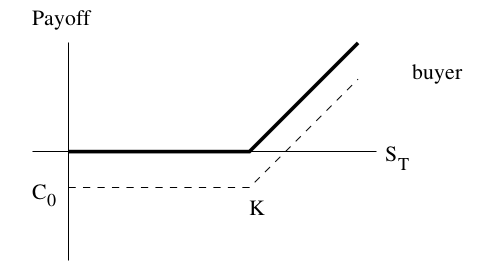
\includegraphics[width=1\linewidth]{Buyer_call} 
		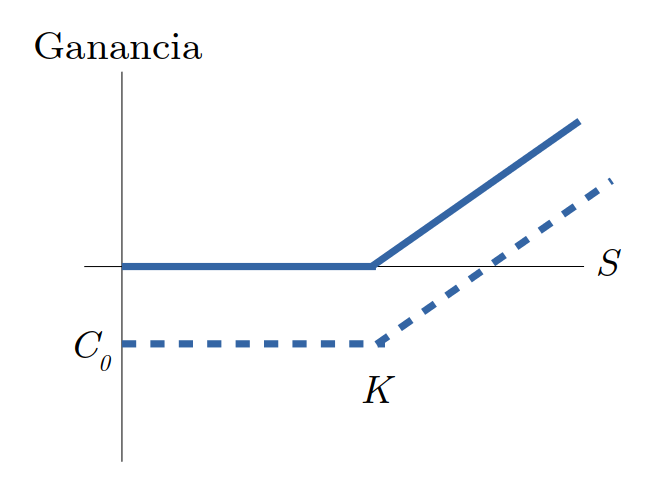
\includegraphics[width=1\linewidth]{Buyer_call_mio} 
		\caption*{Propietario}
		%\label{fig:subim1}
	\end{minipage}
	\begin{minipage}{0.5\textwidth}
		%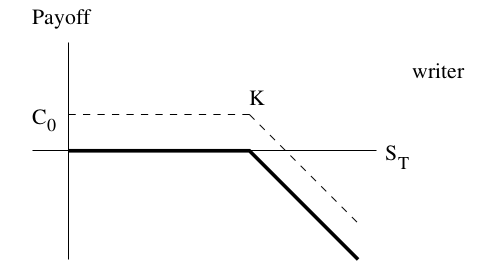
\includegraphics[width=1\linewidth]{Writer_call}
		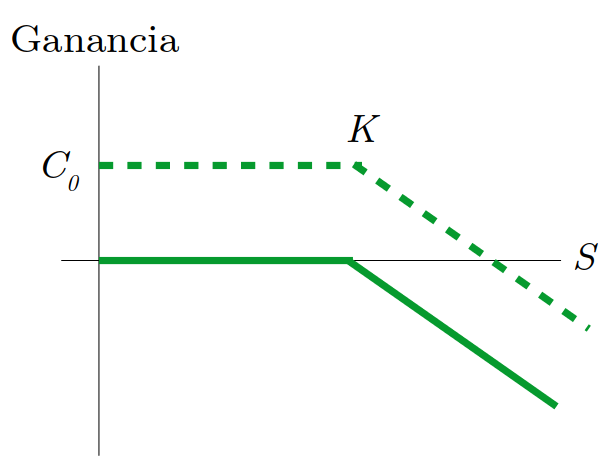
\includegraphics[width=1\linewidth]{Writer_call_mio}
		\caption*{Vendedor}
		
		%\label{fig:subim2}
	\end{minipage}
	\caption{Ganancia opción \textit{call}.}
	\label{graphCall}
\end{figure}

\begin{figure}[h!]
	
	\begin{minipage}{0.5\textwidth}
		\centering
		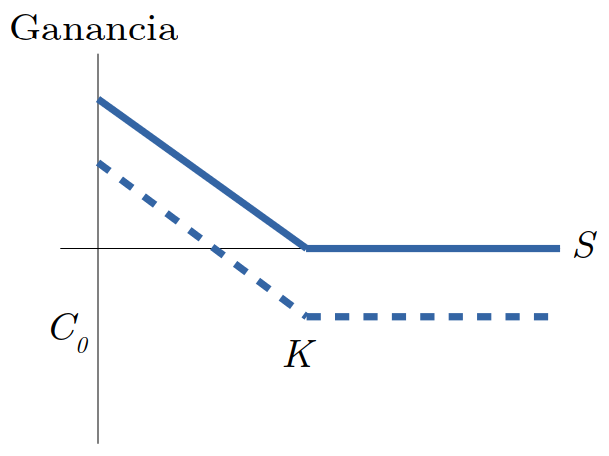
\includegraphics[width=1\linewidth]{Buyer_put_mio} 
		\caption*{Propietario}
		%\label{fig:subim1}
	\end{minipage}
	\begin{minipage}{0.5\textwidth}
		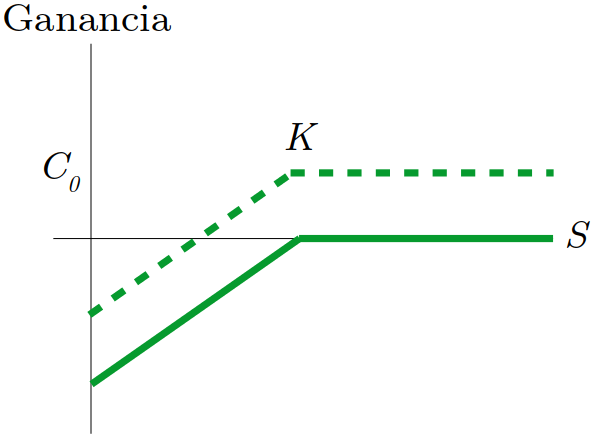
\includegraphics[width=1\linewidth]{Writer_put_mio}
		\caption*{Vendedor}
		%\caption{Tras cuatro iteraciones.}
		
		%\label{fig:subim2}
	\end{minipage}
	\caption{Ganancia opción \textit{put}.}
	\label{graphPut}
\end{figure} 
Uno de los problemas más importantes es determinar de manera única el precio ``justo'' de una opción en un momento determinado para que ambas partes estén de acuerdo. Para más información acerca de conceptos financieros, se pueden consultar \cite{elliot1999mathematics} y el manual para universitarios publicado por la Comisión Nacional del Mercado de Valores que se puede consultar en \url{https://www.cnmv.es/DocPortal/Publicaciones/Guias/ManualUniversitarios.pdf}.\\
